\documentclass[crop,tikz]{standalone}
\usepackage[utf8]{inputenc}
\usepackage{tikz}
\usepackage{pgfplots}
\usepackage{bm}
\pgfplotsset{compat=newest}
\usepgfplotslibrary{groupplots}
\begin{document}
% This file was created by tikzplotlib v0.8.2.
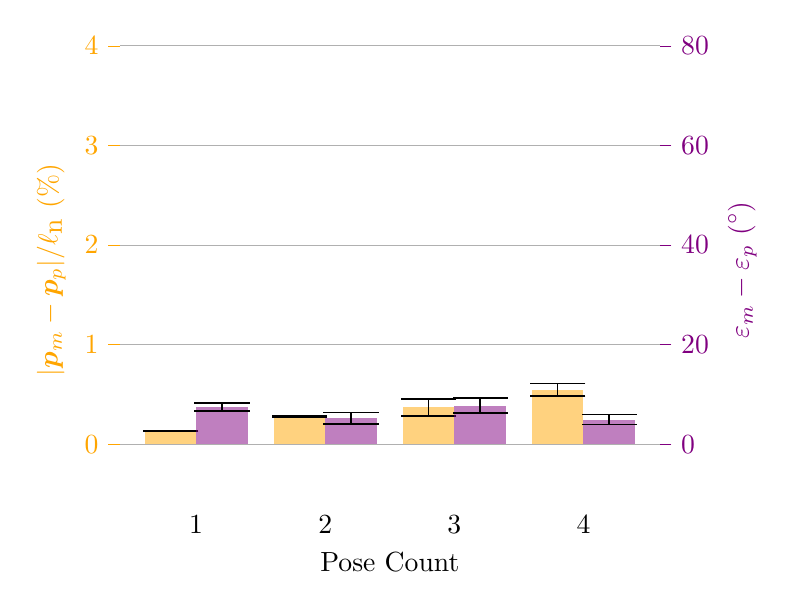
\begin{tikzpicture}
\definecolor{color0}{rgb}{1,0.647058823529412,0}
\definecolor{color1}{rgb}{0.501960784313725,0,0.501960784313725}
\begin{axis}[
anchor=origin,
axis line style={draw=none},
tick align=outside,
tick pos=both,
x grid style={white!69.01960784313725!black},
xmin=-0.59, xmax=3.59,
xtick style={color=black},
xtick style={draw=none},
xtick={0,1,2,3},
xticklabels={ , , , },
y grid style={white!69.01960784313725!black},
ylabel style={color=color0},
ylabel={\(\displaystyle |\bm{p}_m - \bm{p}_p|/\ell_{\textnormal{n}}\) (\%)},
ymin=-0.5, ymax=4,
ytick pos=left,
%ytick pos=right,
ytick style={color=color0},
ytick style={color=color0},
yticklabel style={color=color0}
]
\draw[fill=color0,draw opacity=0,fill opacity=0.5] (axis cs:0,0) rectangle (axis cs:-0.4,0.13171043012063);
\draw[fill=color0,draw opacity=0,fill opacity=0.5] (axis cs:1,0) rectangle (axis cs:0.6,0.279025160919658);
\draw[fill=color0,draw opacity=0,fill opacity=0.5] (axis cs:2,0) rectangle (axis cs:1.6,0.369512572316093);
\draw[fill=color0,draw opacity=0,fill opacity=0.5] (axis cs:3,0) rectangle (axis cs:2.6,0.547564703256519);
\path [draw=black, semithick]
(axis cs:-0.2,0.126838520401977)
--(axis cs:-0.2,0.136582339839284);
\path [draw=black, semithick]
(axis cs:0.8,0.276508249608141)
--(axis cs:0.8,0.281542072231176);
\path [draw=black, semithick]
(axis cs:1.8,0.286237027447019)
--(axis cs:1.8,0.452788117185168);
\path [draw=black, semithick]
(axis cs:2.8,0.48417146707101)
--(axis cs:2.8,0.610957939442029);
\addplot [semithick, black, mark=-, mark size=10, mark options={solid}, only marks]
table {%
-0.2 0.126838520401977
0.8 0.276508249608141
1.8 0.286237027447019
2.8 0.48417146707101
};
\addplot [semithick, black, mark=-, mark size=10, mark options={solid}, only marks]
table {%
-0.2 0.136582339839284
0.8 0.281542072231176
1.8 0.452788117185168
2.8 0.610957939442029
};
\end{axis}
\begin{axis}[
anchor=origin,
axis line style={draw=none},
axis y line=right,
tick align=outside,
tick pos=both,
x grid style={white!69.01960784313725!black},
xlabel={Pose Count},
xmin=-0.59, xmax=3.59,
xtick style={color=black},
xtick style={draw=none},
xtick={0,1,2,3},
xticklabels={1,2,3,4},
y grid style={white!69.01960784313725!black},
ylabel style={color=color1},
ylabel={\(\displaystyle \varepsilon_m - \varepsilon_p\) (\(\displaystyle ^\circ\))},
ymajorgrids,
ymin=-10, ymax=80,
ytick pos=left,
ytick pos=right,
ytick style={color=color1},
ytick style={color=color1},
yticklabel style={color=color1}
]
\draw[fill=color1,draw opacity=0,fill opacity=0.5] (axis cs:0,0) rectangle (axis cs:0.4,7.53603782424437);
\draw[fill=color1,draw opacity=0,fill opacity=0.5] (axis cs:1,0) rectangle (axis cs:1.4,5.27194695848294);
\draw[fill=color1,draw opacity=0,fill opacity=0.5] (axis cs:2,0) rectangle (axis cs:2.4,7.78568683629479);
\draw[fill=color1,draw opacity=0,fill opacity=0.5] (axis cs:3,0) rectangle (axis cs:3.4,4.96860197795693);
\path [draw=black, semithick]
(axis cs:0.2,8.34320854597403)
--(axis cs:0.2,6.72886710251472);
\path [draw=black, semithick]
(axis cs:1.2,6.41193666589046)
--(axis cs:1.2,4.13195725107543);
\path [draw=black, semithick]
(axis cs:2.2,9.32877765972077)
--(axis cs:2.2,6.2425960128688);
\path [draw=black, semithick]
(axis cs:3.2,5.95258311535969)
--(axis cs:3.2,3.98462084055417);
\addplot [semithick, black, mark=-, mark size=10, mark options={solid}, only marks]
table {%
0.2 8.34320854597403
1.2 6.41193666589046
2.2 9.32877765972077
3.2 5.95258311535969
};
\addplot [semithick, black, mark=-, mark size=10, mark options={solid}, only marks]
table {%
0.2 6.72886710251472
1.2 4.13195725107543
2.2 6.2425960128688
3.2 3.98462084055417
};
\end{axis}
\end{tikzpicture}
%% End matplotlib2tikz content %% 
\end{document}